\chapter{Normal Distribution}
Suppose we are in a probability space well approximated by the multivariate normal (Gaussian) distribution of a random variable $x \in \R^n$ with mean $\mu$ and non-singular covariance $\Sigma$:
\marginnote{The $n=1$ example in the introduction is just where where $\mu$ and $\Sigma$ are scalars.}
\begin{align}
P_{\text{normal}}(x;\mu,\Sigma) &= \frac{e^{-\frac{1}{2}(x-\mu)^T \Sigma^{-1} (x-\mu)}}{\sqrt{(2\pi)^n \det{\Sigma}}}  \,,\\
\intertext{where}
\mu_i &= E(x_i)\,,\\
\intertext{and}
\Sigma_{ij} &= E((x_i-\mu_i)(x_j-\mu_j)) \,.
\end{align}

How lucky is some outcome $x$? From the definition:
\begin{align}
L(x)&=|\Omega(x)|+\frac{1}{2}|\omega(x)| \,,\\
\intertext{where}
\Omega(x) =& \left\{ y \in \R^n \middle| P_{\text{normal}}(y) > P_{\text{normal}}(x) \right\} \\
          =& \left\{ y \in \R^n \middle| |\sqrt{\Sigma^{-1}}(y-\mu)| < |\sqrt{\Sigma^{-1}}(x-\mu)| \right\}
\intertext{and}
\omega(x) =& \left\{ y \in \R^n \middle| |\sqrt{\Sigma^{-1}}(y-\mu)| = |\sqrt{\Sigma^{-1}}(x-\mu)| \right\} \,.
\end{align}
Because $\omega(x)$ has no volume in $\R^n$,
\begin{equation}
|\omega(x)|=\int_{\omega(x)} P_{\text{normal}}(y;\mu,\Sigma) \, dy = 0 \,.
\end{equation}

 So
\begin{align}
L(x) &=|\Omega(x)|\\
     &=\int_{\Omega(x)} P_{\text{normal}}(y;\mu,\Sigma) \,dy\,.
\end{align}

\marginnote{$\Sigma$ is symmetric and positive definite, and so is its inverse.  The square-root can be computed as a Cholesky decomposition.  In Scilab, \lstinline[language=Scilab]{z=chol(Sigma)'\\(x-mu)}}
By changing variables to $z=\sqrt{\Sigma^{-1}} (x-\mu)$,
\begin{equation}
L(x) = \int_{|z|<R}  P_{\text{normal}}(z;0,I) \, dz \,,
\end{equation}
\marginnote{\lstinline[language=Scilab]{R=norm(z)}}
where $R = |\sqrt{\Sigma^{-1}} (x-\mu)|$.

This can be evaluated in spherical coordinates:
\begin{align}
\label{eq:normal-luck-as-integral}
L(x)    &=\frac{1}{\sqrt{(2\pi)^{n}}} \int_{0}^{R} \frac{n \pi^{n/2}}{\Gamma(\frac{n}{2}+1)} r^{n-1} e^{-\frac{1}{2} r^2} \, dr \,, \\
    &=\frac{\gamma(n/2,R^2/2)}{\Gamma(n/2)} \,.
\end{align}
\marginnote{\lstinline[language=Scilab]{L=cdfgam("PQ",R^2/2,n/2,1)}}
The last form uses the lower incomplete gamma function and gamma function, defined to be
\begin{align}
\gamma(s,x) &= \int_0^{x} t^{s-1} e^{-t} \, dt \\
\Gamma(s) &= \gamma(s,\infty) \,.
\end{align}
For any value of $n$, but particularly for large values, we find the following approximation to be very good\marginnote{This comes from a Taylor expansion of the log of the integrand in (\ref{eq:normal-luck-as-integral}), and numerical experimentation on the $1/2$ factor.  The expansion is specifically invalid for $n=1$, hence the difference between the general case and the $n=1$ case (\ref{eq:normal-1d-luck}).}:
\marginnote{\lstinline[language=Scilab]{Lapprox=0.5*(1+erf(R-sqrt(n-1/2)))}}
\begin{equation}
\label{eq:normal-luck-approx}
L(x) \approx \frac{1}{2}\left[1+\erf(|\sqrt{\Sigma^{-1}} (x-\mu)|-\sqrt{n-1/2})\right] \,.
\end{equation}
\begin{figure}
  \caption{Exact (blue) vs approximate (red) luck for normal distribution for $n=1$, $10$, and $100$.}
  \centering
    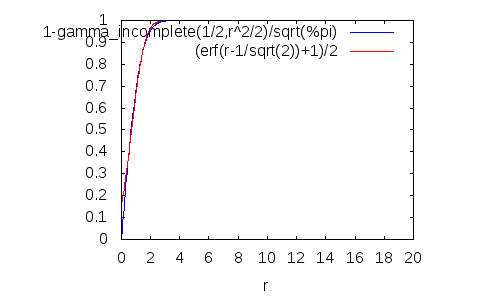
\includegraphics[width=0.75\textwidth]{img/luck1}
    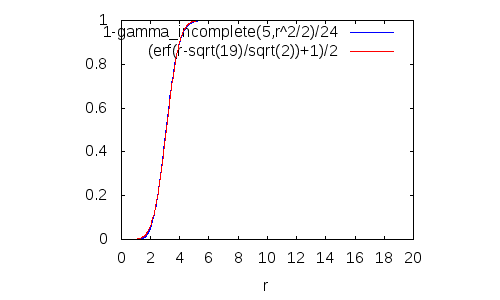
\includegraphics[width=0.75\textwidth]{img/luck10}
    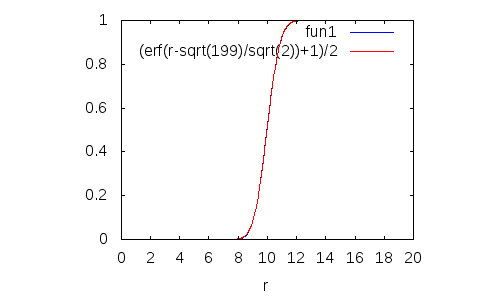
\includegraphics[width=0.75\textwidth]{img/luck100}
\end{figure}

Not only is this result pretty, it is very useful.  Suppose we have distribution parameters $\mu$ and $\Sigma$, and would like to know if they fit actual observations.  A traditional approach requires a large sample to estimate $\mu$ and $\Sigma$, but we don't need this, nor do we need to assume that the distribution is normal.  We just need to ask if the observations are surprising (lucky or unlucky).  In large dimensions, numerical experiments suggest one sample is in most cases sufficient to establish practical certainty (probability of error less than $10^{-15}$).
\begin{table}
\caption{\label{tab:normal}Luck from two randomly generated distributions $\mu^{(x)}$ and $\mu^{(y)}$ uniformly chosen in $[0,1]^{100}$, and $\Sigma^{(x)}, \Sigma^{(y)}$ are transposed squares of random $100 \times 100$ matrices.  In each row, $x$ is  a sample from the $\mu^{(x)},\Sigma^{(x)}$, normal distribution, and $y$ is from the $\mu^{(y)},\Sigma^{(y)}$ distribution.  The actual values of $x$ and $y$ are not given, since they are very large (100 numbers each) and uninteresting.}
\begin{tabular}{|S[table-format=2.10]|S[table-format=2.10]|S[table-format=2.10]|S[table-format=2.10]|}
\multicolumn{1}{c}{$L^{(x)}(x)$} &
\multicolumn{1}{c}{$L^{(y)}(x)$} &
\multicolumn{1}{c}{$L^{(x)}(y)$} &
\multicolumn{1}{c}{$L^{(y)}(y)$} \\
\hline
0.5014172020 & 1.0000000000 & 1.0000000000 & 0.8381802641 \\
0.7314212665 & 1.0000000000 & 1.0000000000 & 0.2392581432 \\
0.9825630339 & 1.0000000000 & 1.0000000000 & 0.2716955127 \\
0.0334550807 & 1.0000000000 & 1.0000000000 & 0.4213206259 \\
0.6894299340 & 1.0000000000 & 1.0000000000 & 0.0744616557 \\
0.7363975937 & 1.0000000000 & 1.0000000000 & 0.2940507284 \\
0.3045212967 & 1.0000000000 & 1.0000000000 & 0.7078490147 \\
0.2311115744 & 1.0000000000 & 1.0000000000 & 0.2903130932 \\
0.5852477199 & 1.0000000000 & 1.0000000000 & 0.6369022028 \\
0.2145529261 & 1.0000000000 & 1.0000000000 & 0.2689897874
\end{tabular}
\end{table}

\begin{figure}
  \caption{Histograms of 10,000 luck values in the same distributions as table~\ref{tab:normal}.  Upshot: $y$ values in the $x$ distribution are viewed as extremely lucky and vice-versa, while they are have uniform luck in their own respective distributions.}
  \centering
    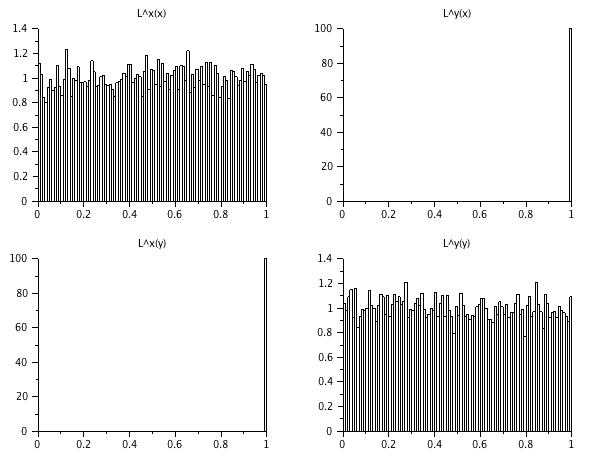
\includegraphics[width=0.75\textwidth]{img/normal}
\end{figure}

\subsection{Combining Normal Luck}
The approximate result (\ref{eq:normal-luck-approx}) leads to a rule for combining (normal) luck:  Suppose there are two independent normal distributions parameterized by $\mu^{(x)}$ , $\Sigma^{(x)}$ of dimension $n_x$, and $\mu^{(y)}$, $\Sigma^{(y)}$ of dimension $n_y$.  What is the luck of a single combined observation $(x,y)$?
\begin{align}
L(x,y) &\approx \frac{1}{2}\left[1+\erf(\sqrt{R_x(x)^2+R_y(y)^2}-\sqrt{n_x+n_y-\frac{1}{2}}) \right] \,,
\intertext{where}
R_x(x) &= \erf^{-1}(2L_x -1)-\sqrt{n_x-\frac{1}{2}} = \sqrt{\left(\Sigma^{(x)}\right)^{-1}} \left(x-\mu^{(x)}\right) \,, \\
R_y(y) &= \erf^{-1}(2L_y -1)-\sqrt{n_y-\frac{1}{2}} = \sqrt{\left(\Sigma^{(y)}\right)^{-1}} \left(y-\mu^{(y)}\right) \,.
\end{align}

The approximations above, which in the limit are exact, lead to the following natural definition:
\begin{definition}{Luck-adjusted $z$-score.}  For any distribution (not just a normal distribution) with finite mean $\mu=E(x)$ and finite positive definite covarience $\Sigma=E((x-\mu)(x-\mu)^T)$, where $x$ and $\mu$ are $n$-dimensional column vectors, it is natural to associate an observation $x$ with the {\em luck-adjusted $z$-score}:
\begin{equation}
z_L = \left|\sqrt{\Sigma^{-1}} (x-\mu)\right|-\sqrt{n-\frac{1}{2}} \,.
\end{equation}
\end{definition}

The luck-adjusted $z$-score from two independent experiments can be combined into one overall score with:
\begin{equation}
\begin{split}
z_L^{A \times B}=&\sqrt{\left(z_L^A+\sqrt{n_A-\frac{1}{2}}\right)^2+\left(z_L^B+\sqrt{n_B-\frac{1}{2}}\right)^2}\\
&-\sqrt{n_A+n_B-\frac{1}{2}} \,.
\end{split}
\end{equation}

Similarly, $k$ repeated independent experiments can be combined with
\begin{equation}
\begin{split}
z_L^{A^k}=&\sqrt{\sum_{i=1}^{k}{\left(z_L^{A_i}-\sqrt{n_A-\frac{1}{2}}\right)^2}} \\
         &-\sqrt{k\cdot n_A - \frac{1}{2}} \,.
\end{split}
\end{equation}

If the combined dimension $n$ is large enough that the overal distribution is well approximated by the normal distribution, then the luck associated with the overall set of observations is well approximated by the {\em normal luck},
\begin{equation}
L_N = \frac{1}{2}\left[1+\erf(z_L)\right] \,.
\end{equation}

If the distribution is in fact normal, the luck can be computed exactly via,
\begin{equation}
L=\frac{\gamma(\frac{n}{2},\frac{1}{2}(z_L+\sqrt{n-\frac{1}{2}})^2)}{\Gamma(n/2)} \,.
\end{equation}
There is less than a $0.01$ difference between $L_N$ and $L$ for $n \geq 22$.

Combining luck-adjusted $z$-scores is very useful for understanding the implications of multiple experiments.  If the model is good, the luck-adjusted $z$-score will to stay small (within $\pm 6$) as you combine the outcomes of more experiments.  If it tends to get large or small, there is something wrong in the model.  If $z_L$ tends to negative infinity, this seems to be an indication of a non-stochastic process (it is being gamed), and if $z_L$ tends to positive infinity, the estimates for $\mu$ and/or $\Sigma$ are wrong.  The publication of $z_L$ and $n$ for experimental results would be very useful for meta analysis, and $L_N$ or $L$ would be a value much easier to interpret for a lay reader.

\subsection{Scilab Reference Code}

The listings in figures \ref{fig:mnprobln}-\ref{fig:mnapproxluck} give Scilab functions for basic luck calculations for multivariate normal distributions.

\begin{figure}
\caption{\label{fig:mnprobln}Scilab listing to compute the natural log of the probability of multivariate normal outcomes.  $x$ is a $n_{\text{dim}} \times n_{\text{samps}}$ of outcomes, $\mu$ is a $n_{\text{dim}} \times 1$ column vector of the means, and $\Sigma$ is a $n_{\text{dim}} \times n_{\text{dim}}$ covariance matrix.  The result {\tt lnp} is a $1 \times n_{\text{samps}}$ row vector.}
\lstset{language=Scilab}
\begin{lstlisting}
function lnp=mnprobln(x,mu,Sigma)
  [dim,nsamps]=size(x);
  sigma=chol(Sigma)';
  z=sigma\(x-mu*ones(1,nsamps));
  R2=sum(z.^2,'r');
  lnp=-R2/2-(dim/2*log(2*%pi)+...
       sum(log(diag(sigma))));
endfunction
\end{lstlisting}
\end{figure}

\begin{figure}
\caption{\label{fig:mnluck}Scilab listing to efficiently compute the luck of multivariate normal outcomes.  $x$ is a $n_{\text{dim}} \times n_{\text{samps}}$ of outcomes, $\mu$ is a $n_{\text{dim}} \times 1$ column vector of the means, and $\Sigma$ is a $n_{\text{dim}} \times n_{\text{dim}}$ covariance matrix.  The result $L$ is a $1 \times n_{\text{samps}}$ row vector of the luck associated with each outcome.}
\lstset{language=Scilab}
\begin{lstlisting}
function L=mnluck(x,mu,Sigma)
  [dim,nsamps]=size(x);
  one=ones(1,nsamps);
  sigma=chol(Sigma)';
  z=sigma\(x-mu*one);
  R2=sum(z.^2,'r');
  L=cdfgam("PQ",R2/2,dim/2*one,one);
endfunction
\end{lstlisting}
\end{figure}

\begin{figure}
\caption{\label{fig:mnapproxluck}Like {\tt mnluck} in figure~\ref{fig:mnluck}, but approximates luck via (\ref{eq:normal-luck-approx}).}
\lstset{language=Scilab}
\begin{lstlisting}
function L=mnapproxluck(x,mu,Sigma)
  [dim,nsamps]=size(x);
  sigma=chol(Sigma)';
  z=sigma\(x-mu*ones(1,nsamps));
  R=sqrt(sum(z.^2,'r'));
  L=0.5*(1+erf(R-sqrt(dim-0.5)));
endfunction
\end{lstlisting}
\end{figure}

